% replace all text with your own text.
% in this template few examples are mention
\chapter{Methodology}
\label{ch:method} % Label for method chapter

\subsubsection{Data Collection}

The ISOT Fake News Dataset serves as the foundation for this research endeavor, comprising articles categorized into real and fake news. Through meticulous collection efforts, articles were sourced from reputable platforms like Reuters.com for truthful content and flagged unreliable sources for fake news articles. The dataset's temporal focus on articles primarily from 2016 to 2017 aligns with a period marked by significant political discourse, making it particularly relevant for studying misinformation dynamics.

Consisting of two CSV files, "True.csv" and "Fake.csv," the dataset offers over 12,600 articles each, providing a rich and diverse collection for analysis. Each article within the dataset includes essential information such as the article title, text, publication date, and categorization as real or fake news. By retaining certain characteristics of fake news articles, such as punctuation and mistakes, the dataset aims to authentically reflect the nature of misinformation encountered in real-world contexts, ensuring its relevance and utility for research purposes.

 \begin{figure}

     \centering
     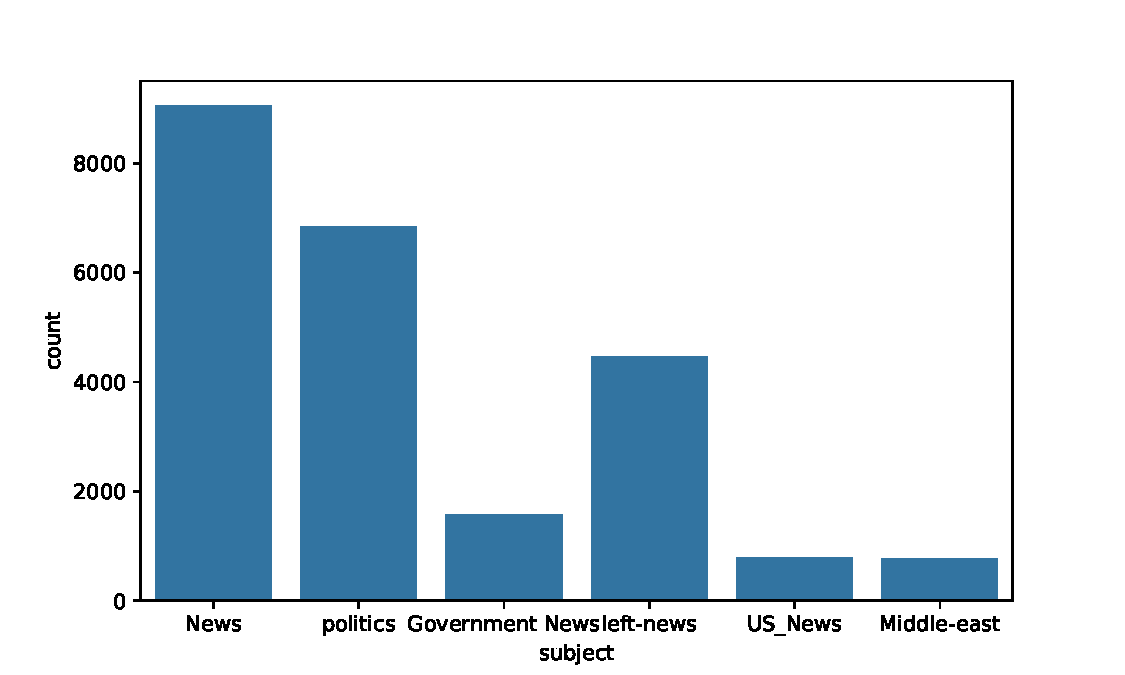
\includegraphics[width=1\linewidth]{figures/FakeNewCategories.pdf}
     \caption{Fake News Categories}
     \label{fig:enter-label}
 \end{figure}

\begin{figure}
    \centering
    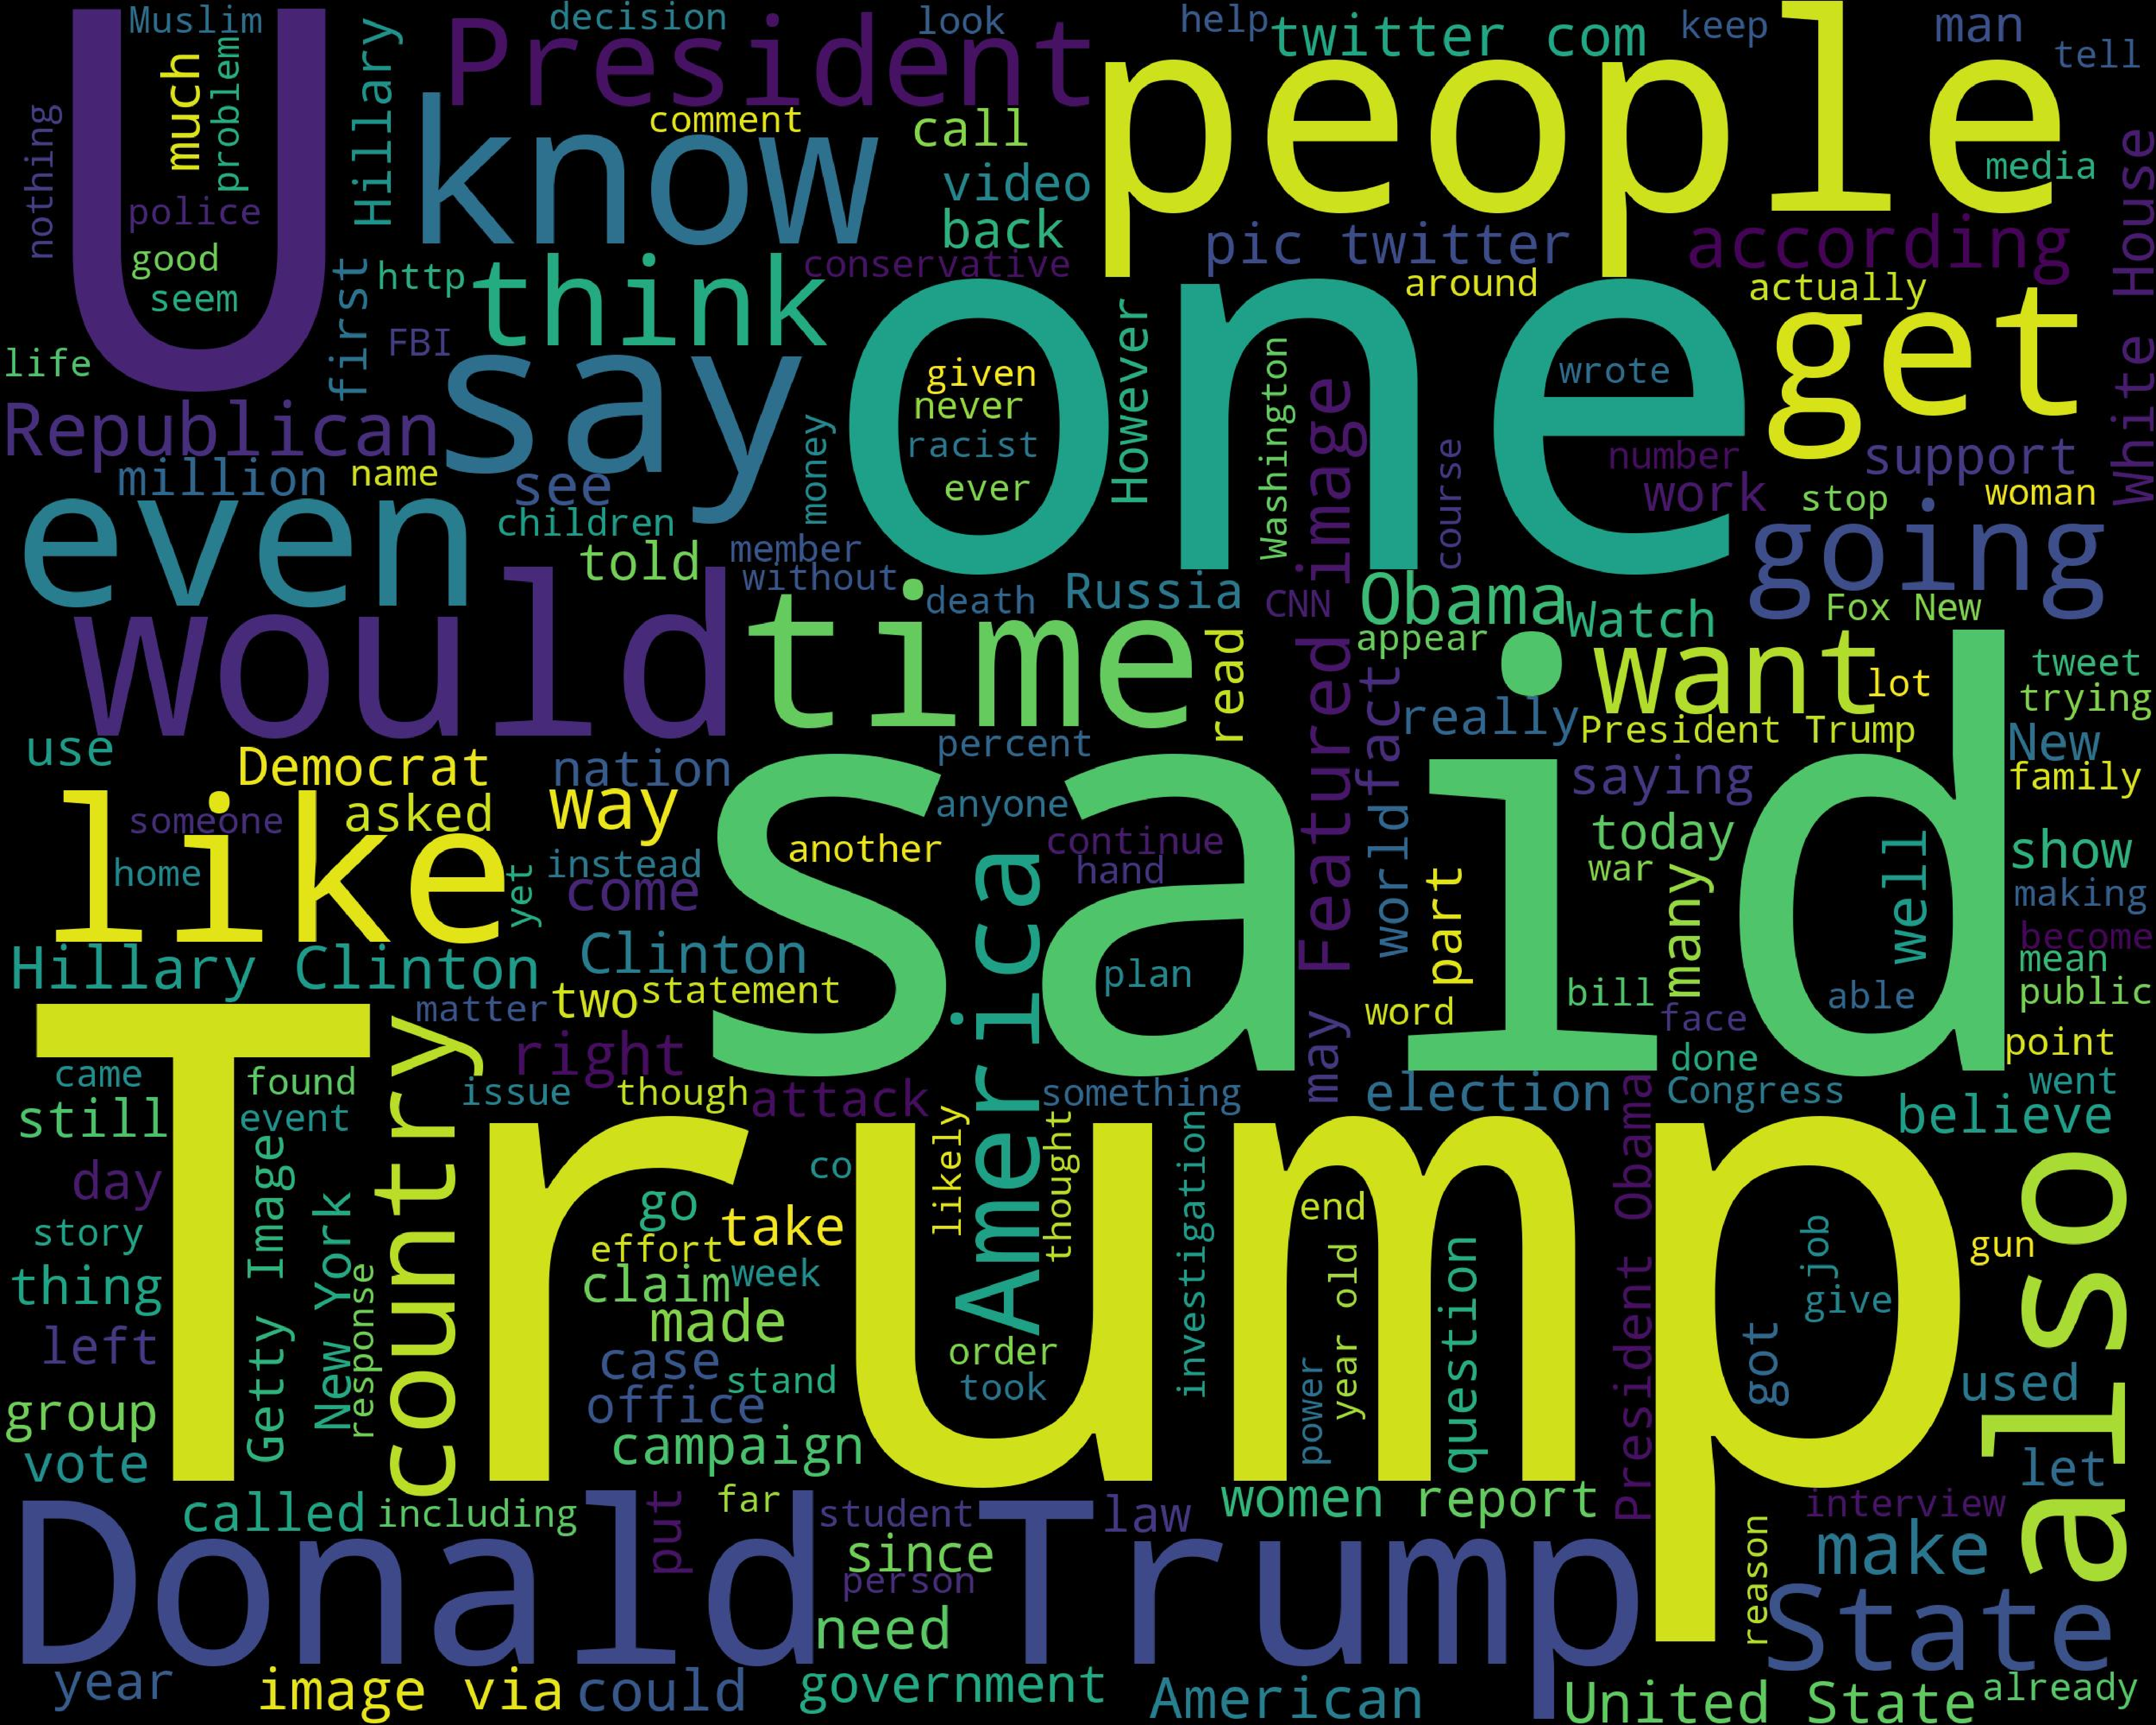
\includegraphics[width=0.75\linewidth]{figures/fakenews_wordcloud.pdf}
    \caption{Fake News - word Cloud}
    \label{fig:enter-label}
\end{figure}


 
\subsubsection{{Data Preprocessing}}
 In the text preprocessing phase, several operations are conducted to refine the dataset for subsequent analysis. Initially, class labels are assigned to distinguish between real and fake news articles, with real articles labeled as class 1 and fake articles as class 0. Next, the title and text content of each article are combined into a single cohesive body to streamline the text processing pipeline. This consolidation enhances the effectiveness of subsequent natural language processing (NLP) tasks by providing a unified textual representation for analysis.

Furthermore, certain attributes that do not contribute significantly to the analysis are removed from the dataset. Specifically, the subject field, which differs between real and fake articles, is dropped, along with the date, title, and publisher information for real articles. This pruning of extraneous attributes streamlines the dataset and focuses attention on the essential text content and class labels. Finally, the processed real and fake datasets are merged into a single dataframe, enabling comprehensive analysis and modeling of the combined dataset. The resultant dataframe, denoted as 'df,' encapsulates the consolidated dataset, ready for further exploration and modeling.

\subsubsection{{Feature Engineering}}
In the feature engineering process, the raw text data is preprocessed and transformed into numerical representations suitable for training machine learning models. Initially, the text is tokenized and cleaned to remove punctuation, stopwords, and other irrelevant characters using the NLTK library. This preprocessing step ensures that the text data is in a standardized format and free from noise that could potentially interfere with the learning process. Subsequently, Word2Vec embeddings are generated using the Gensim library, which learns distributed representations of words by capturing their semantic and syntactic relationships. These word embeddings encode rich semantic information and enable the modeling of word context, similarity, and association within the textual data.

Furthermore, the tokenized text sequences are converted into numerical sequences using a tokenizer, where each word is mapped to a unique numerical identifier. These numerical representations facilitate the input of text data into deep learning models such as recurrent neural networks (RNNs) or convolutional neural networks (CNNs). To ensure uniform input dimensions, the text sequences are padded or truncated to a fixed length, allowing for efficient processing within the neural network architecture. By transforming the raw text into numerical sequences and embedding them into a continuous vector space, the feature engineering phase lays the groundwork for training robust machine learning models capable of capturing intricate patterns and relationships within the textual data.

\subsubsection{Model Selection}

The chosen neural network architecture for this research project integrates an embedding layer initialized with pre-trained Word2Vec embeddings, followed by an LSTM layer and a dense layer for binary classification. By leveraging pre-trained embeddings, the model can effectively capture semantic information and contextual relationships within the news articles. This initialization ensures that words with similar meanings are represented closer in the embedding space, facilitating the model's ability to understand the underlying semantics of the text. Subsequently, the LSTM layer is incorporated to handle the sequential nature of the input data, enabling the model to capture temporal dependencies and long-term patterns within the text. LSTM networks are particularly well-suited for processing sequential data and have demonstrated effectiveness in various NLP tasks, making them a suitable choice for this classification task.

The addition of a dense layer with a sigmoid activation function allows the model to perform binary classification, predicting the likelihood of a news article being real or fake. By outputting a probability score between 0 and 1, the model can effectively differentiate between the two classes. The binary cross-entropy loss function is employed to optimize the model parameters during training, while accuracy serves as the evaluation metric to assess the model's performance. This architecture strikes a balance between capturing semantic relationships, modeling sequential data, and performing binary classification, thereby demonstrating its efficacy in classifying news articles while considering the complex linguistic structure and contextual nuances present in the text data.


\subsubsection{Model Training and Evaluation}
The dataset was split into training and testing sets using the train test split function, with a default ratio of 75\% for training and 25\% for testing. The model was then trained on the training data for a total of 7 epochs, during which the neural network's parameters were adjusted iteratively to minimize the loss between the predicted and actual class labels. The training process involved monitoring the model's performance on a validation subset, comprising 30\% of the training data, to prevent overfitting and ensure generalization.
